\documentclass{article}
\usepackage[T1]{fontenc}
\usepackage[utf8]{inputenc}
\usepackage{amsfonts}
\usepackage{amssymb}
\usepackage{amsmath}
\usepackage{graphicx}
\usepackage{url}

\author{Hjalti Leifsson (hjaltil13@ru.is)\\Jóhann Örn Bjarkason (johannob01@ru.is)}
\title{\textbf{Project Discovery}}
\begin{document}
\maketitle
\section{Introduction}\label{sec:introduction}

In this report we discuss the progress of our final project, \emph{Project Discovery}. In section~\ref{sec:time} we list the hours we have spent so far on the project in total and for each of us. In section~\ref{sec:burndown} we show the status of the burndown chart at this point, after four sprints have been completed. In section~\ref{sec:backlog} we go over the sprint backlogs of the sprints we've done so far and show the burndown charts for each sprint we have completed. Lastly in section~\ref{sec:retrospectives} we summarize our sprint planning and retrospective meetings. 
\section{CCP and background}\label{sec:ccp}

\subsection{Background}

We worked on this project in conjunction with CCP Games. The project was a continuation of work done by Reykjavík University graduates Gunnar Þór Stefánsson and Þór Adam Rúnarsson. They worked on it as their final project for the spring semester of 2015. They continued their work with a grant from Rannís during the summer of 2015. Gunnar had to leave the project in the beginning of July and Hjalti Leifsson replaced him. 

When the project began, a user interface design had been decided, and the game had around half of that design already implemented. The design can be seen on figure \ref{fig:PD}.

\begin{figure}[H]
	\centering
	\graphicspath{ {./graphics/} }
    \centerline{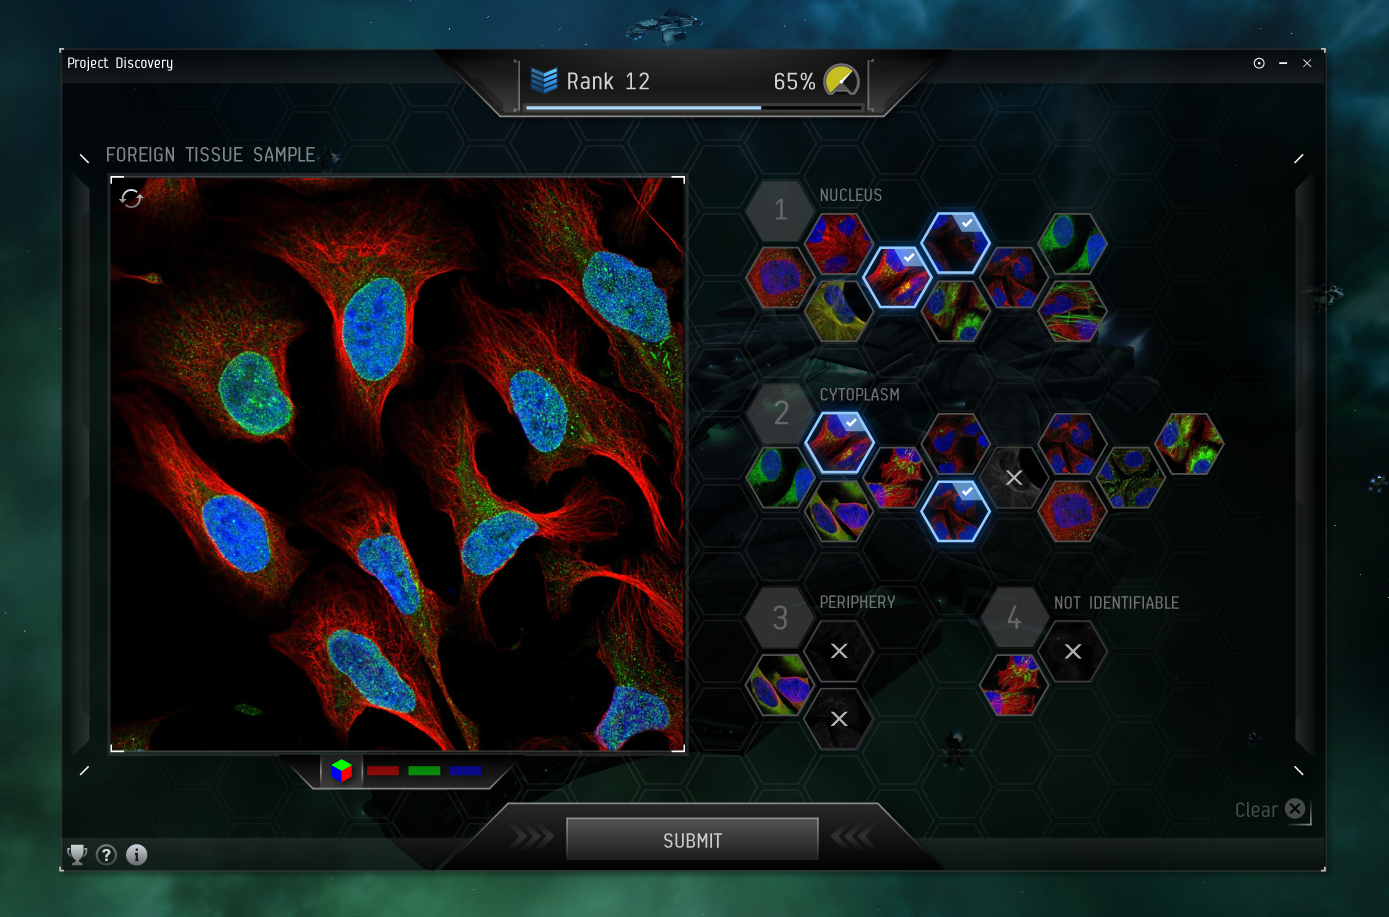
\includegraphics[scale=0.35]{PD.png}}
    \caption{\label{fig:PD}The design of the UI as the project began}
\end{figure}

The game already had a few features implemented, such as players being able to receive images, selecting their appropriate categories and submitting their classifications. A simple rewarding system was also already in place, rewarding players with in game currency (ISK), experience points (XP) and loyalty points (LP) when players submitted a solution. The reward was based on their score for the image they just classified, but since those images were 'training images', we knew the solution and could grade the player on that. However, that needed to be changed later on because when the client got an image that we did not know the solution for, no reward was given. Finally, a rudimentary tutorial phase was implemented, but it was too small and needed to be expanded to improve new player experience.

\subsection{CCP Games}

CCP develops massively multiplayer online games and has become one of the leading companies in that field. It is dedicated to make original, cutting edge games. CCP is best known for their groundbreaking massively multiplayer online role-playing game (MMORPG) \emph{EVE Online}, which has enjoyed great popularity and received critical acclaim, winning Game of the Year three times from \href{http://www.mmorpg.com/}{MMORPG.com}. In addition to \emph{EVE Online}, CCP also develops \emph{DUST 514\textsuperscript{\textregistered}}, an innovative, free-to-play, massively multiplayer online first-person shooter for the PlayStation\textsuperscript{\textregistered}3, and \emph{EVE: Valkyrie™}, a multiplayer spaceship dogfighting shooter, both set in the EVE Universe. CCP was founded in Reykjavík Iceland in 1997. Its headquarters have since recided there but it also has locations in Atlanta, Newcastle and Shanghai. Further information can be found at \href{http://www.ccpgames.com/}{CCPGames.com}.

CCP provided us with facilities to work on the project, and their game \emph{EVE Online} accomodates Project Discovery within its game universe. We had a project manager, Pétur Örn Þórarinsson, from CCP to help us work with the company. 

\subsection{EVE Online}
\emph{EVE Online} is the game which plays host to \emph{Project Discovery}. It is based in a science fiction space setting. Players of the game have a great deal of freedom in how they choose to play and don't need to follow pre-defined missions. They can engage in many different activities such as mining, piracy, manufacturing, trading, exploration and combat (both player versus environment and player versus player). \emph{Project Discovery} fits smoothly into the game as players can solve tasks from anywhere in the game. To access \emph{Project Discovery}, players go through the menu and select it, and a new window opens up on the game screen.

\section{Game with a purpose}\label{sec:gwap}
\subsection{MMOS}

\section{Project Discovery}\label{sec:project_discovery}
In this section we discuss the status of the game as it was at the beginning of the project, and outline the general architecture of the game.

\subsection{Beginning status of the game}
When the project began, the newest user interface design had been decided, (see figure \ref{fig:PD}), and the game had around half of that design already implemented. Some features had already been implemented, such as players being able to receive images, selecting their appropriate categories and submitting their classifications. A simple rewarding system was already in place, rewarding players with in game currency (ISK), experience points (XP) and loyalty points (LP). A rudamentary tutorial phase was already in place, but needed reforming.\\

\begin{figure}[H]
	\centering
	\graphicspath{ {./graphics/} }
    \centerline{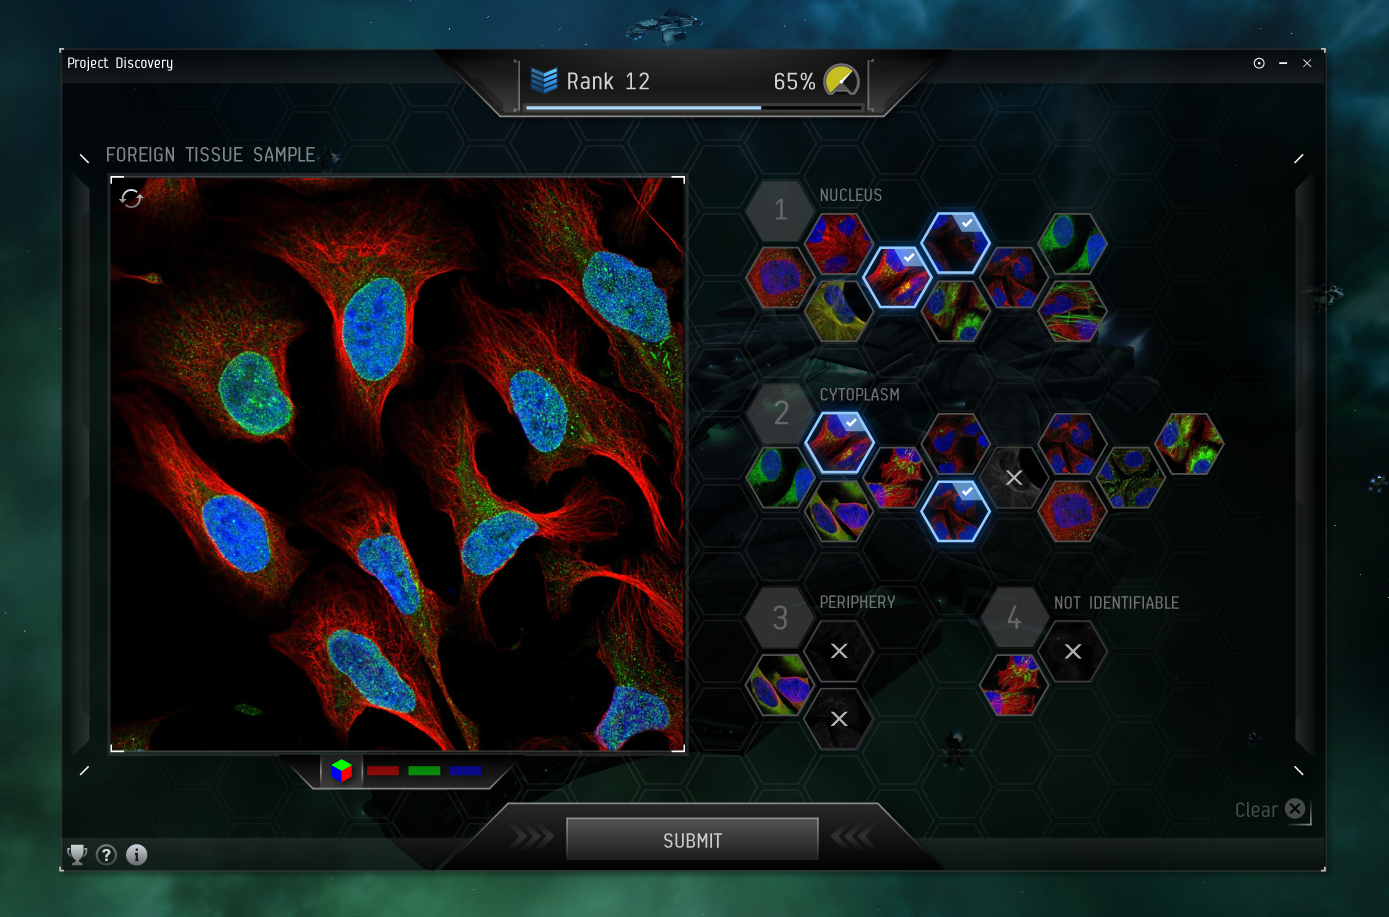
\includegraphics[width=15cm]{PD.png}}
    \caption{\label{fig:PD}The design of the UI when the project began}
\end{figure}

\subsection{Architecture}
%Talk about architecture, show a photo?
\section{Expected outcome}\label{sec:expected_outcome}


Two main outcomes are expected by the end of the project. One is to implement the remaining features of \emph{Project Discovery}, and launch it on the \emph{EVE Online} test server, \emph{Singularity}. The other is to develop and launch a website dedicated to \emph{Project Discovery} that details its progress and player statistics, as well as informs the players and general public about it.\\

These are the main remaining features that we expect to be able to finish for this project:
\begin{itemize}
  \item A training phase where players get easy tasks and a few categories to solve.
  \item A detailed rewarding system, where players complete daily challenges for further rewards.
  \item A leaderboard, where players compete to be the best of the best.
  \item A detailed view of the history of player submissions, where each player can see what submission changed their score.
\end{itemize}

We also need to clear up a few things regarding authorization, optimization, player statistics tracking and how our client will be able to connect to the external MMOS API.\\

After release on the test server (or before, it is undecided), our task is to develop a website to launch along with the mini-game. At this point no development or design has been done on the website and only very basic discussion has taken place on the content of it, so the web development part of the project is likely to change and expand in scope. What we know currently is that it will contain information about \emph{Project Discovery} and it will in some way show the progress the \emph{EVE} players are making with the research, for an example how many pictures have been analyzed and how many more need to be analyzed.


%%%%%%%%%%%%%%%%%%%%%%%%%%%%%%%%%%%%%%%%%%%%%%%%%%%%%%%%%%%%%%%%%%%%%%%%%%%%%%%%%%%%%%%%%%%%%%%%%%%%%%%
%\section*{Description}
%As stated above, this project started in January 2015 and the first few months of the project served as the final project at Reykjavík University by Gunnar Þór Stefánsson and Þór Adam Rúnarsson. They continued their work with a grant from Rannís. Gunnar had to leave the project in the beginning of July and Hjalti replaced him so Hjalti was already well up to speed when this semester started. 
% 
%To explain our part in the project we first go over what has been done already and the bigger picture of the project. The project is a so called Citizen Science project. Citizen Science (also known as crowd-sourced science) is scientific research conducted by many amateur or non-professional scientists. A lot of research must be performed by humans since no computational alternative exists and Citizen Science can help speed up research of that kind. 
%
%MMOS (Massively Multiplayer Online Science), which is one of the companies behind the project, is trying to find new ways to conduct Citizen Science by mobilizing players in online video games to take part in the research. The idea is to make the research a seamless part of the gameplay and offer in-game rewards to encourage players to take part. This project, which is called \emph{Project Discovery} within \emph{EVE Online}, focuses on creating a game with a purpose in the \emph{EVE Universe} which will serve as a platform for research tasks. In this incarnation \emph{Project Discovery} will involve players in identifying protein patterns in images of cells and then classifying them in the correct category. This is done in conjunction with \href{http://www.proteinatlas.org/subcellular}{The Human Protein Atlas} which provides the images to be analyzed. In the future Project Discovery could be used for other similar research tasks within the EVE universe.
%
%\section*{Current status of the project}
%
%When we took over the project in the beginning of the semester a lot of the work on the mini-game had already been done.
%The game has an API from MMOS it can talk to in order to receive images for players, and score them based on their performance (in-game it is called "Accuracy Rating"). Players can therefore receive tasks and make selections on that task, based on available categories. They can then submit the task, and get-in game rewards and an updated accuracy score. Players receive a message, thanking them for their contribution, after each submitted task. They also receive in-game experience. Players level up with experience and can figuratively reach an endless level, there is no set limit. The highest level, for which you receive rewards for achieving, is level 100. Players also receive milestone titles for reaching certain level thresholds, such as: "Novice Analyst".
%
%\begin{figure}[H]
%	\centering
%    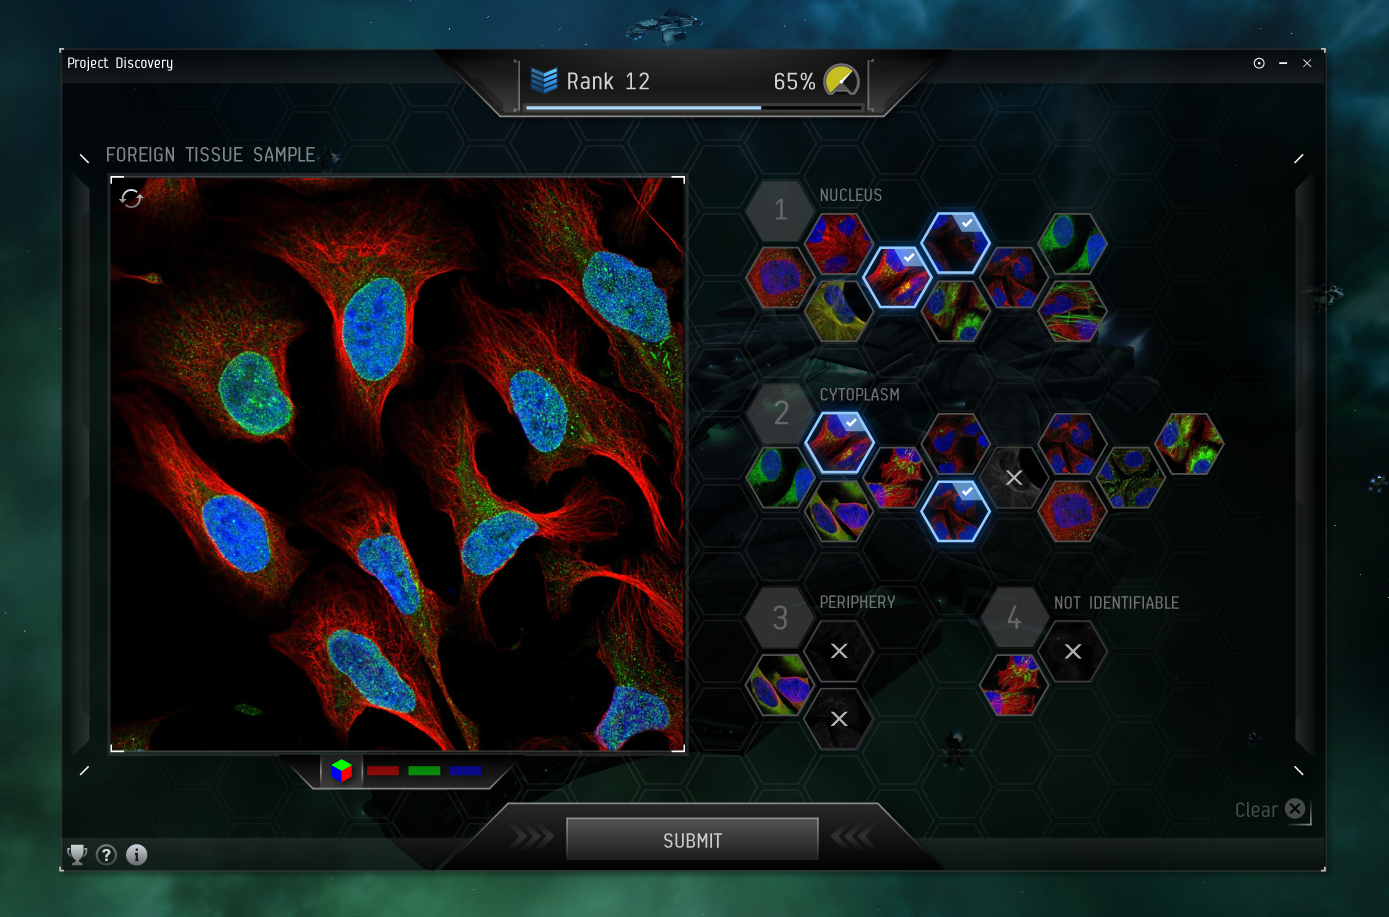
\includegraphics[width=15cm]{PD.png}
%    \caption{\label{fig:PD}This is the design of the UI at this point}
%\end{figure}
%
%\section*{Outcome of the project}
%
%Two main outcomes are expected by the end of the project. One is to implement the remaining features of \emph{Project Discovery}, and launch it on the \emph{EVE Online} test server, \emph{Singularity}. The other is to develop and launch a website dedicated to \emph{Project Discovery} that details its progress and player statistics, as well as informs the players and general public about it.\\
%
%These are the main remaining features that we expect to be able to finish for this project:
%\begin{itemize}
%  \item A training phase where players get easy tasks and a few categories to solve.
%  \item A detailed rewarding system, where players complete daily challenges for further rewards.
%  \item A leaderboard, where players compete to be the best of the best.
%  \item A detailed view of the history of player submissions, where each player can see what submission changed their score.
%\end{itemize}
%
%We also need to clear up a few things regarding authorization, optimization, player statistics tracking and how our client will be able to connect to the external MMOS API.\\
%
%After release on the test server (or before, it is undecided), our task is to develop a website to launch along with the mini-game. At this point no development or design has been done on the website and only very basic discussion has taken place on the content of it, so the web development part of the project is likely to change and expand in scope. What we know currently is that it will contain information about \emph{Project Discovery} and it will in some way show the progress the \emph{EVE} players are making with the research, for an example how many pictures have been analyzed and how many more need to be analyzed.
%
%\section*{About the companies (from the project proposal)}
%CCP is a leading independent developer of massively multiplayer games, and has
%been praised for its artistry, game design and unique player-driven, infinitely scalable
%storytelling narratives. In addition to \emph{EVE Online}, CCP also develops \emph{DUST 514\textsuperscript{\textregistered}}, a
%groundbreaking, free-to-play, massively multiplayer online first-person shooter for
%the PlayStation\textsuperscript{\textregistered}3, and \emph{EVE: Valkyrie™}, a multiplayer spaceship dogfighting shooter, both set in the EVE Universe. Founded and headquartered in Reykjavik,
%Iceland, in 1997, CCP is privately held, with additional offices in Atlanta, Newcastle,
%and Shanghai. For more information, visit \href{http://www.ccpgames.com/}{ccpgames.com}.\\
%
%MMOS is a privately held start-up company from Switzerland specializing in the field
%of citizen science. The company was founded in 2014 by Attila Szantner and
%Bernard Revaz. Mr. Szantner has a long history in the field of IT, amongst other
%projects being one of the creators of iwiw.hu (the Hungarian “Facebook” which at its
%height \href{http://en.wikipedia.org/wiki/IWiW}{reached more than 4 million users}). Mr.
%Revaz has 15 years of research history in physics (University of Geneva, University
%of California, EPLF).\\
%
%
%CADIA is a highly innovative interdisciplinary centre at Reykjavík University that
%explores and extends the relationship between humans and intelligent machines
%through deep understanding and modeling of human behaviour, design of real-time
%sensing and decision making mechanisms, and extensive prototyping and evaluation
%methodology. CADIA’s projects have received numerous international awards and
%honours, including being three times winners of the international General Game
%Playing (GGP) competition, two times recipients of the Kurzweil Award for Artificial
%General Intelligence (AGI) and placing fourth at the international Autonomous
%Underwater Vehicle (RoboSub) competition. CADIA contains 8 faculty members and
%over 40 research staff and students. Learn more at \href{http://cadia.ru.is/}{cadia.ru.is}.
\end{document}
